\chapter{相关技术综述}
这是章节标题。
注:一般而言,标题不要比小节标题更小,即不要出现1.2.3.4这种标题(本模板支持此类标题,即Subsubsection)。

\section{漏洞挖掘技术}
漏洞挖掘指用自动化或半自动化技术对软件进行本身进行静态,动态分析,检测其是否存在安全漏洞的过程~\cite{liujian2018}。随着软件规模扩大,软件功能种类多样化,安全漏洞其种类也在不断增多,不同漏洞的产生原因不同,利用方式也不同,一种漏洞挖掘技术不能适用于所有漏洞,因此在实践中,人们会在软件开发的各个阶段应用不同类型的技术,本文将这些技术的应用场景主要分为三类:
\begin{itemize}
    \item  白盒测试:也成为静态测试,通常发生在软件编码阶段,对应用程序的源代码或对源码编译产生的二进制文件进行安全性审计,从而发现漏洞。该场景下的技术由于获取了源代码信息,也被称为源码扫描或静态扫描,其可以获得较高的代码覆盖率,发现更多的漏洞,但由于无法运行而产生大量误报,它也是本文系统的应用场景。
    \item 黑盒测试:通常发生在软件测试和运行阶段,对应用程序动态运行,并输入数据,分析程序反应从而发现漏洞。适用于该场景的技术可以在程序只暴露接口的情况下展开测试,因此应用广泛,同时动态运行程序使其获得更低的误报,甚至产生漏洞利用报告,但由于如今应用程序复杂,自动化测试技术往往无法覆盖所有的代码逻辑。
    \item 灰盒测试:介于白盒和黑盒之间的一种测试,这一场景下的技术往往通过软件插桩或是逆向工程,不但关注程序输入输出信息,还可以了解部分程序内部逻辑。因此具备上述两种测试的优点,许多黑白盒测试技术稍加改造也可以变为灰盒测试技术,但由于其终究还是需要获取程序本身,以及需要动态运行,适用性比纯黑百盒测试弱。
\end{itemize}

在漏洞挖掘技术发展早期,每一种技术往往只能应用于一种特定场景,但随着研究者的不断完善和改进,如今一种技术也可以适用于多种场景,并且技术本身也产生了相互组合,对其正交分类较为困难,本章就目前常用的漏洞挖掘技术进行分类并分别进行简要介绍~\cite{liujian2018,meihong2009}。


% 需要写java的常见漏洞吗?
\subsection{基于代码分析的漏洞挖掘技术}
这一类漏洞挖掘技术侧重于对程序代码本身进行分析,同时对漏洞产生原理进行建模,将程序分析结果结合漏洞模型发掘漏洞,主要用于白盒测试场景。主要有词法分析技术,数据流分析技术,形式化分析技术和符号执行技术。\\
\vspace{1cm}
\subsubsection{词法分析技术}
词法分析技术是最简单的一类漏洞挖掘技术,其主要思想是将代码文本与一直归纳好的缺陷模式进行匹配,以此发现漏洞。由于其不深入分析程序结构和语义,往往只能挖掘较为简单的一类漏洞,并且存在相当高的误报率,在实际场景下应用较少,但由于其思想简单,适用性很广,目前也还存在类似工具,如:MobSF~\footnote{\url{https://github.com/MobSF/Mobile-Security-Framework-MobSF}},cobra~\footnote{\url{https://github.com/WhaleShark-Team/cobra}}。\\

\subsubsection{数据流分析技术}
数据流分析是一种按程序执行路径模拟数据流动的一种分析技术,通过分析数据在流动时的取值或状态,来发现程序中的安全漏洞,其在白盒,灰盒和黑盒测试都有体现。

在数据流分析过程中,存在过程内分析和过程间分析,过程内分析主要对函数内分析而过程间的分析主要处理跨函数分析。
对于过程内分析,根据其对程序路径的分析精度,数据流分析可以分为流不敏感分析,流敏感分析和路径敏感分析。流不敏感的数据流分析只是按代码行号从上而下进行分析;流敏感分析会首先产生程序的控制流图(CFG, Control Flow Graph),再按照CFG的拓扑排序正向或逆向的分析;路径敏感信息不仅考虑到语句的先后顺序,还会考虑语句的可达性,即会沿实际可行的路径进行分析。
过程间分析首先构造程序的调用图(CG, Call Graph),接着遍历图中的函数进行过程内分析,当遇到其他函数时,若已分析过,则直接使用分析结果向下分析,若未分析过,则跟进该函数,再次进行过程内分析,并且将分析结果保存。

数据流分析能够一定程度上理解程序语义,是一种比词法分析技术更为精确的一类分析技术,其关键在于准确的计算程序的数据流,此外,本文使用的污点分析技术作为数据流分析的一种特例,将在下文单独一章进行介绍。\\

\subsubsection{形式化方法分析技术}
形式化方法分析主要思想是将软件代码性质进行形式化描述,再判断该描述是否满足漏洞特征的一类分析方法~\cite{B:automatedTheoremProving},其中定理证明技术是形式化代码分析技术的主要代表。

%https://firmianay.gitbooks.io/ctf-all-in-one/doc/5.0_vulnerability.html
%Automated Theorem Proving in Software Engineering
%https://github.com/leanprover/lean2
定理证明技术将漏洞存在(或不存在)定义为一定理,再将源程序代码特征转化为数学表达形式,最后对数学表达进行逻辑推理,若定理存在性得以证明,则漏洞存在(或不存在),即漏洞挖掘过程类似于数学上的定理证明过程。主要代表性工具有infer~\footnote{\url{https://fbinfer.com/}}~\cite{atp:infer}, ESC/Java~\cite{atp:escjava}和saturn~\cite{atp:saturn}。

该技术作为一种使用严格的数理逻辑推理作为检测手段的技术,具有极低的误报率,但由于其需要针对特定漏洞构建数学条件,其过程需要大量的人工参与,有的漏洞甚至难以用断言结构表达,适用于死循环,资源泄露,空指针等问题,对新漏洞的扩展性不高,同时,如何将大规模程序应用于形式化方法分析也成为工业界亟待解决的问题。 \\

\subsubsection{符号执行技术}
符号执行技术是一种将程序执行可达性问题转化为约束求解问题,并以此进行漏洞挖掘的技术~\cite{sym:sum},代表性工具有angr~\footnote{\url{http://angr.io/}},DART~\cite{sym:dart}, CUTE~\cite{sym:cute}, EXE~\cite{sym:exe}和KLEE~\cite{sym:klee}。
% https://www.youtube.com/watch?v=mffhPgsl8Ws
% https://blog.csdn.net/wcventure/article/details/86773290
%Symbolic Execution for Software Testing: Three Decades Later

具体来说,符号执行包含一个符号状态表$\sigma$和一个符号路径约束$PC$,开始时,$\sigma=\empty, PC=true$,每读取一条语句,就将变量抽象为约束求解中的变量、常量或他们的表达式放入$\sigma$中,特别的,当遇到条件判断$if(e)$时,将if分支的$PC$更新为$PC \wedge \sigma(e)$,将else分支的$PC'$更新为$PC\wedge \neg\sigma(e)$,随后使用约束求解器求解$PC$和$PC'$,如果约束不满足,则停止对该分支的解析,因为该分支不可达。当符号执行遇到程序崩溃、预先定义的漏洞语句、或是程序正常退出时,整个分析停止,同时可以计算可以到达停止点的输入。

符号执行可以分析程序中的控制流,覆盖更多的代码,另外其使用约束求解模拟执行程序的方法也有效降低了误报率,但传统符号执行严重依赖于约束求解器的能力,例如,若约束求解器不能处理非线性计算,或是整个程序中存在无法分析的第三方库,那么整个分析将无法继续。为解决这些问题,研究者们提出了动态符号执行的想法~\cite{sym:dart,sym:cute,sym:exe,sym:klee},但其在实际应用中仍不是很广泛,主要原因在于其需要大量计算资源,甚至在处理大规模程序时,出现的路径爆炸问题会导致约束求解无法产生结果。\\

\subsection{基于模糊测试的漏洞挖掘技术}
模糊测试是一种通过构造大量非预期输入,同时观察软件运行反馈来发现软件漏洞的方法~\cite{fuzzingstateofart}。

由于其不需要了解程序内部具体实现,不论是Web应用还是二进制程序,其都是一种非常受欢迎的技术。
其关键在于如何构造能够引发软件漏洞的输入,对于Web应用来说,扫描器会针对每个漏洞(如SQL注入,XSS等)准备若干个(或若干组)可能会引发漏洞的输入模式,接着爬虫程序会爬取网站所有URL,在扫描到符合条件的URL时,将这些输入模式整合进HTTP报文中,将其发送给服务器,若服务器返回符合漏洞特征,则报告程序存在漏洞,主要的工具有AWVS~\footnote{\url{https://www.acunetix.com/vulnerability-scanner/}},Netsparker~\footnote{\url{https://www.netsparker.com/}}和ZAP~\footnote{\url{https://www.zaproxy.org/}}。
学术界更热衷于对二进制程序的模糊测试技术进行改进~\cite{artoffuzz},为了构造能够到达更深层代码的输入,研究者们提出了通过代码覆盖率制导的模糊测试技术,即在第一轮使用测试人员指定的输入,在以后的测试中,对能够产生新路径的输入进行变异,再将变异后的输入进行测试,其代表性的工具有AFL~\footnote{\url{http://lcamtuf.coredump.cx/afl/}}和libFuzzer~\footnote{\url{https://llvm.org/docs/LibFuzzer.html}}。

模糊测试作为一种能够得到漏洞利用的一种漏洞挖掘技术,在黑盒和灰盒场景下应用广泛,但由于目前程序日益复杂,该漏洞挖掘技术很难测试隐藏在复杂状态已经条件分支下的代码块,导致程序覆盖率不高,即其具有低误报,高漏报的特点。

\section{污点分析}
%https://www.k0rz3n.com/2019/03/01/%E7%AE%80%E5%8D%95%E7%90%86%E8%A7%A3%E6%B1%A1%E7%82%B9%E5%88%86%E6%9E%90%E6%8A%80%E6%9C%AF/
%https://github.com/firmianay/CTF-All-In-One/blob/master/doc/5.5_taint_analysis.md
%http://www.jos.org.cn/html/2017/4/5190.htm
%http://www.jos.org.cn/html/2019/2/5581.htm
污点分析属于数据流分析的变种,通过判断关键操作的数据(如调用危险函数的参数)是否可被用户操控,来判断程序是否安全性漏洞~\cite{taint:wanglei}。由于其能考虑程序上下文,并且有较强的可解释性——安全工程师可以通过跟踪污点传播树判断是否存在安全问题,因此其也成为了挖掘Web或Android漏洞较为常用的技术,很多白盒扫描器都使用了技术,如:Find-sec-bugs~\footnote{\url{https://www.microfocus.com/en-us/products/static-code-analysis-sast/}},Fortify~\footnote{\url{https://www.microfocus.com/en-us/solutions/application-security}}和LGTM~\footnote{\url{https://lgtm.com/}}。\\

\subsection{污点分析原理}

\subsubsection{污点分析三要素}
污点分析主要有三个组成要素:污点信息的产生点(source)、污点信息的汇聚点(sink)和污点信息的清洁点(clean)。

\begin{itemize}
	\item 产生点(Source):污点的产生点往往是用户输入的数据,比如Web应用中读取URL参数的函数,顾名思义,这些函数调用后的返回值被标记为污点——攻击者可以操控的数据点。
	\item 汇聚点(sink):检查点是程序的一些敏感操作,如调用数据库查询语句,或是将数据返回到网页,如果这些操作的操作数据是污点,那么意味着操作可被攻击者利用,即程序存在漏洞。
	\item 清洁点(clean):清洁点通常是对污点进行消除的一类操作,如SQL注入、XSS中的过滤函数。清洁点是污点传播准确性的重要保证,不能识别清洁点即会引发污点过污染问题。
\end{itemize}
这些三要素主要是通过安全从业人员根据经验手动标记,而在学术界也存在同统计或机器学习产生点和汇聚点的研究。\\

\subsubsection{污点传播过程}
污点传播分为静态污点传播和动态污点传播,两者区别在于静态污点传播利用程序代码进行污点传播,而动态污点传播则需要通过程序的实际运行进行传播,由于本文关注于白盒测试情景,故只介绍静态污点传播方法,而在下一子章节会介绍动态传播的优劣势。

在定义好以上三要素之后,污点传播分析法会与数据流分析一样,对程序进行过程内分析和过程间分析。

过程内分析包括了显式流分析和隐式流分析,显示流分析即通过分析变量的数据依赖关系进行数据传播,而隐式分析则是指考虑控制依赖进行数据传播。虽然攻击者确实可以利用控制依赖操作数据进行攻击,但由于其分析复杂且会产生大量误报,在工程领域常常只做数据流依赖的显示分析,因此本文主要讨论显式流分析。

\begin{figure}[htb]
	\centering
	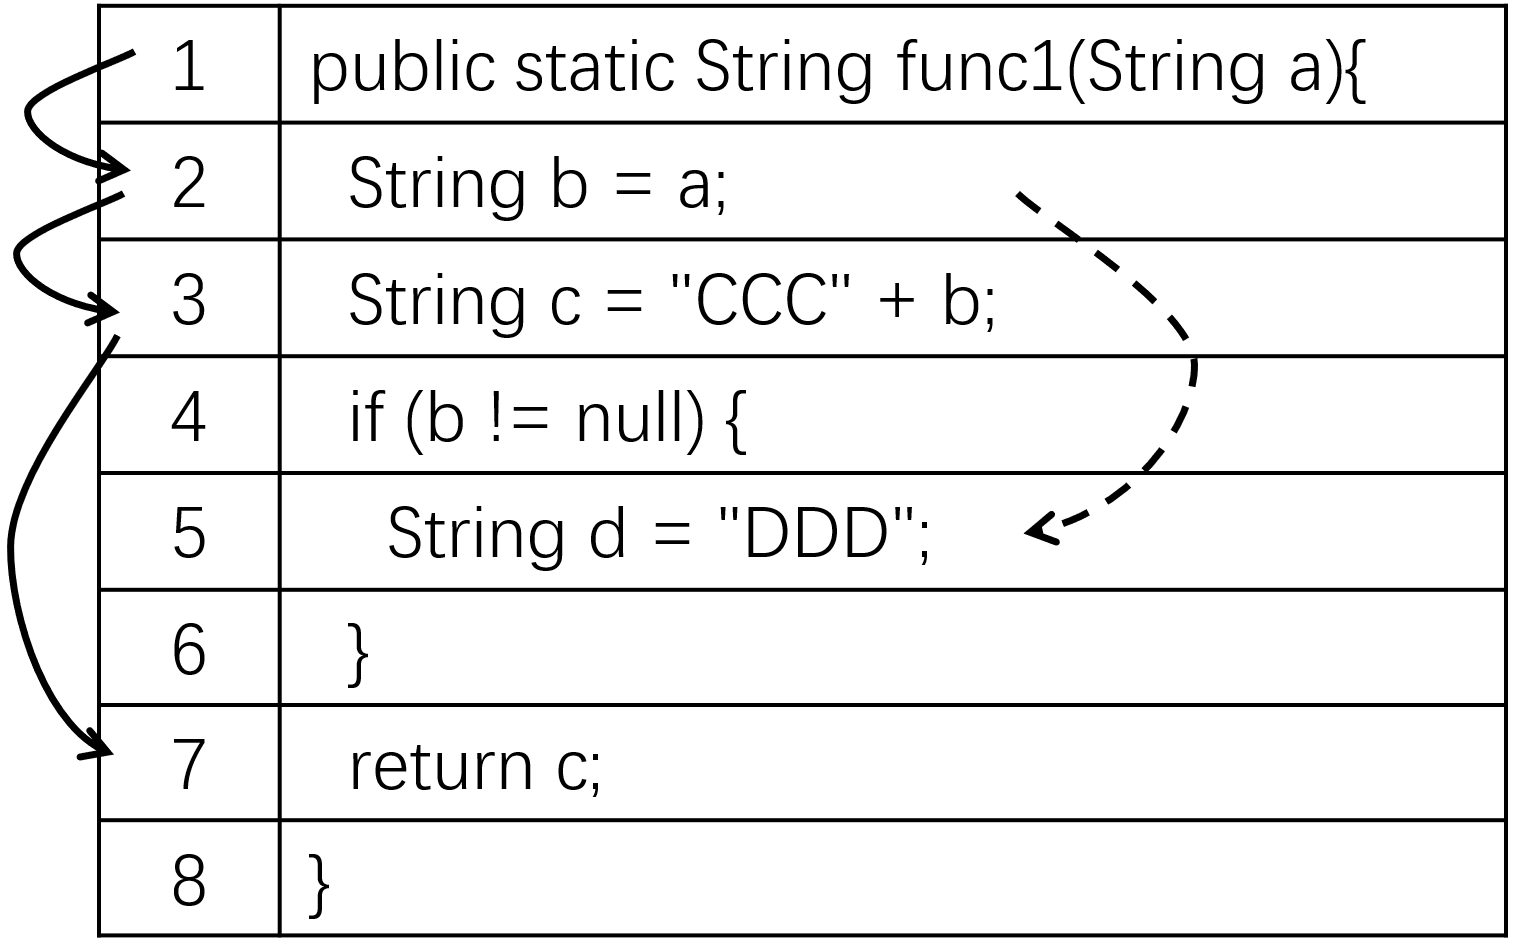
\includegraphics[width=0.5\linewidth]{FIGs/chapter2/internal_taintflow.png}
	\caption{过程内污点分析}\label{internalflow}
\end{figure}

如图~\ref{internalflow}所示,首先假设变量$a$为污点变量,实线箭头表示了显示污点传播路径,而虚线箭头表示了隐式污点传播路径,同时该图也说明了过程内污点传播基本思想,即从上至下遍历数据流图,若未标记的变量依赖于污点变量,则新变量也被标记为污点变量。

由于现代程序存在着复杂的函数调用,因此除了进行过程内分析,还需要进行过程间分析。其分析首先构造函数调用图(Call Graph),接着搜索存在产生点的函数,对于每一个存在产生点的函数,自顶向下分析。遇到函数调用时,跟进被调函数,进行过程内污点分析,将分析结果表达为$\left\langle f, S, r\right\rangle$的函数摘要,其中$f$包含函数本身摘要信息(类名方法名和函数签名),$S$指调用过该函数后被污染的变量集合,$r$取值0或1,标记函数返回值是否被污染;接着根据函数摘要,再进行过程内分析,如此往复直至分析完函数所有代码块或是污点传布到汇聚点报告漏洞。
\begin{figure}[htb]
	\centering
	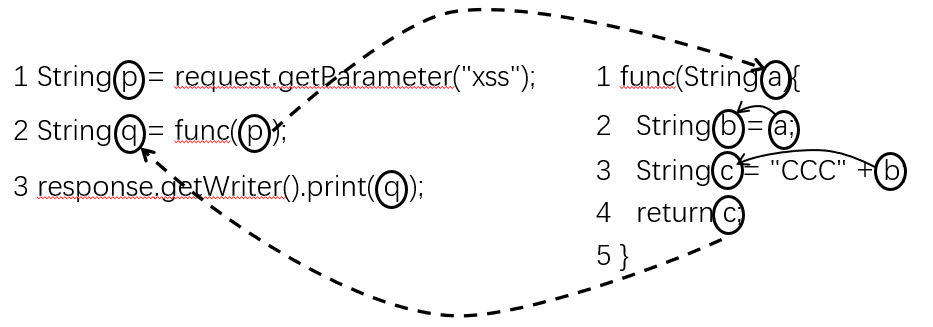
\includegraphics[width=0.7\linewidth]{FIGs/chapter2/external_taintflow.png}
	\caption{过程间污点分析}\label{externalflow}
\end{figure}

如图~\ref{externalflow}所示,分析过程从左侧函数开始,因为其找到了一处产生点——\textit{request.getParameter("xss")},于是将污点传递到变量\textit{p},接着调用函数\textit{func(p)},于是对函数\textit{func}做过程内分析,得到其函数摘要,$\left\langle func, p, 1\right\rangle$,即其可以将污点返回,于是回到调用者的函数内,变量\textit{q}被标记为污点,又因为第三行存在一处汇聚点——\textit{response.getpriter.print()},并且参数为污点,于是报告此处有漏洞,并且根据汇聚点可以判断该漏洞是一个XSS漏洞。\\

\subsection{污点分析的优势和不足}
污点分析能够对程序上下文有一定理解,往往能产生误报率相对较低以及可解释的漏洞报告,因此,本文也选择该技术产生初步的漏洞扫描结果。

然而,污点传播仍有可能发生误报,以下通过简单示例来说明。

\begin{figure}
	\centering
	\subfigure[污点传播难以处理容器类型]{
		\label{taintcase1}
		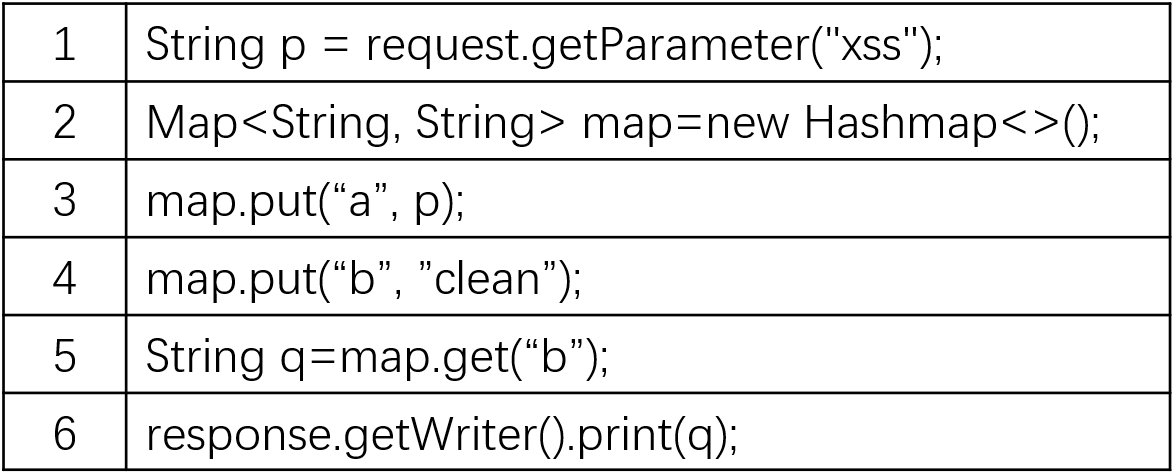
\includegraphics[width=0.4\textwidth]{FIGs/chapter2/tpcase1.png}}
	% \hspace{0.1in}
	\subfigure[污点传播难以分析控制流]{
		% \label{fig:subfig:b} %% label for second subfigure
		\label{taintcase2}
		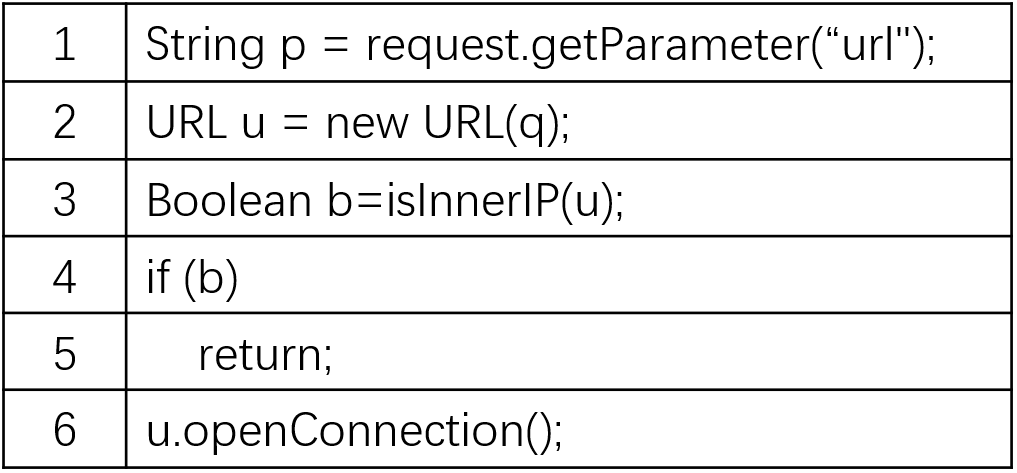
\includegraphics[width=0.4\textwidth]{FIGs/chapter2/tpcase2.png}}
	\subfigure[污点传播难以分析控制流]{
		% \label{fig:subfig:b} %% label for second subfigure
		\label{taintcase3}
		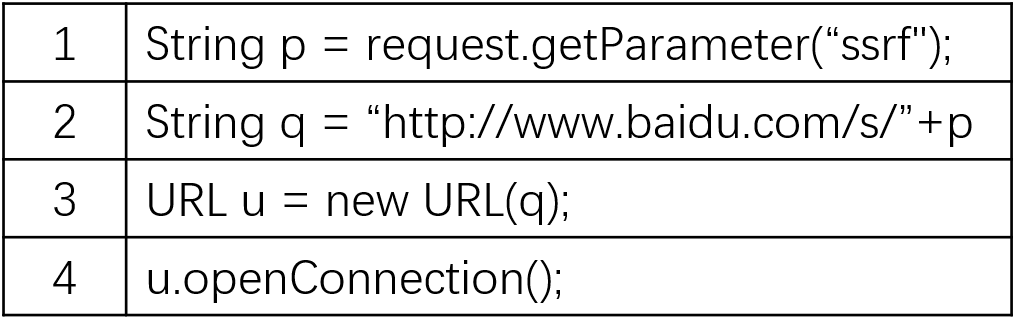
\includegraphics[width=0.4\textwidth]{FIGs/chapter2/tpcase3.png}}
	\subfigure[污点传播难以分析控制流]{
		% \label{fig:subfig:b} %% label for second subfigure
		\label{taintcase4}
		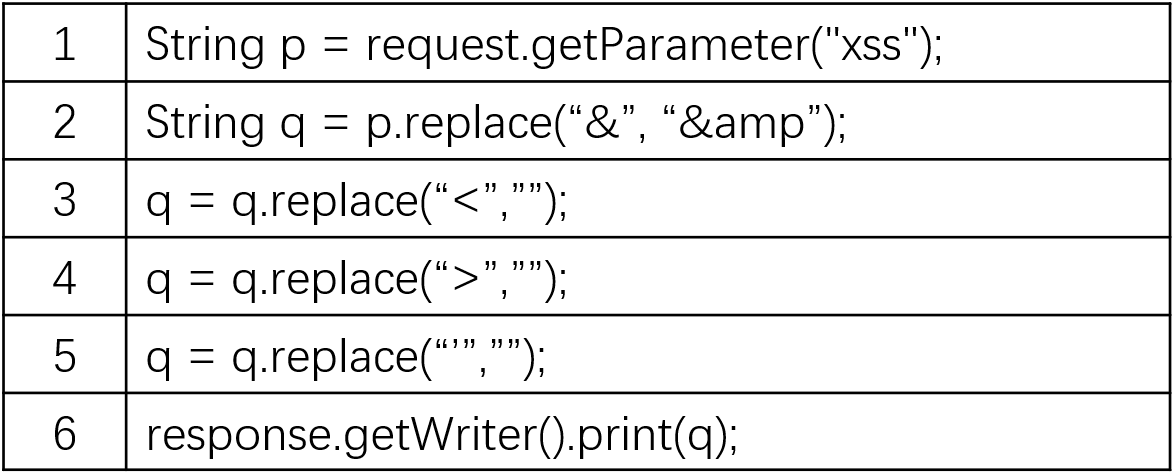
\includegraphics[width=0.4\textwidth]{FIGs/chapter2/tpcase4.png}}
	\caption{污点传播的不足}
	\label{fig:rq3} %% label for entire figure
\end{figure}
首先,污点传播对容器类型无法做很好处理,如图~\ref{taintcase1}所示,当污点传入容器类型时(在此例子中为\textit{map}),静态污点传播只能将这类变量的传播规则设为传播/不传播污点,从而造成过污染/欠污染,就如图所示,若设为\textit{map}传播污点,由于案例实际从容器中取出的是没有污点的变量,即过污染,而若设为不传播,若\textit{q}取出了参数\textit{p},那么又导致了欠污染。动态污点传播虽然解决了这一问题,但是由于其使用条件复杂,且无法用于静态分析,本文暂不讨论。

此外,由于静态污点传播对控制流没法做很好的处理,如图~\ref{taintcase2}所示,在第三行,程序已经对可能产生的SSRF漏洞进行了处理,即如果是内部地址的话则直接返回,但是不论是考虑显式流还是隐流,污点传播不能处理这一类判断。

再者,对于特殊触发条件的漏洞,污点传播无法很好处理,如图~\ref{taintcase3}所示,在第二行,因为SSRF要求攻击者能够操控主机名,所以即使用户输入的污点变量拼接在了一个正常网站之后,程序也不会出现SSRF的问题,而按照污点传播分析法,毫无疑问它会报告这段程序存在SSRF漏洞。

最后,不论是动态污点传播还是静态污点传播,其对污点清洁点的识别能力几乎为零,如图~\ref{taintcase4}所示,程序已经对潜在的XSS攻击做出的处理——即在第2-5行对用户输入的特殊符号进行替换和过滤,但是污点传播并不能识别这些清洁点,导致误报。

正是因为存在这些不足,本文将在下文引入程序切片技术和LSTM来降低误报率。\\

\section{程序切片技术}
\subsection{程序切片技术介绍}

\subsection{后向程序切片的优势}

\section{词嵌入技术}
(后期可能会改为文档嵌入技术,先不写)

\section{LSTM算法}
\subsection{LSTM原理介绍}
\subsection{LSTM的优势}

\section{本章小结}